\clearpage
\twocolumn[{%
\rqparent
\subsection{Decision accuracy against the training tokens of the language}
\label{app:rq02_da_vs_train_tokens}

\noindent\begin{minipage}[t]{0.485\textwidth}
\vspace{0pt}
\paragraph{Research Question.} \emph{Does a language's BPB rank the design variants like the 1.7B reference once the proxy has seen enough of that language?}

\paragraph{Setup.} We measure the DA-goal of per-language BPB against the tokens of that language the model has seen. DA-goal is the share of design pairs that a checkpoint orders like the final 1.7B checkpoint. We use every data build at seed 1904: the proxies 90M--1B at each evaluated tenth of their run, and the early checkpoints of the 1.7B run. Each of the 50 trained languages gives one task, its BPB. A language's pairs are the pairs of design variants that train it, on any number of design axes, with at least three pairs per language. A point is the mean over languages at one size and tenth, placed at the tokens of the language seen.
\end{minipage}\hfill
\begin{minipage}[t]{0.485\textwidth}
\vspace{0pt}
\begin{rqfinding}
\textbf{1. The 600M rung is the outlier, not the smallest proxy.} At the final checkpoint DA-goal is 0.95 at 90M and 175M, 0.91 at 350M, 0.73 at 600M and 0.92 at 1B (standard error over languages 0.006--0.011). (Figure~\ref{fig:app_rq02_da_vs_train_tokens}.)
\\
\\
\textbf{2. Tokens seen do not set the level.} The 90M proxies read 0.92 at their first tenth on 0.008 B tokens of a language, while the 600M proxies read 0.73 at their final on 0.50 B, and 1B at its first tenth (0.08 B) reads 0.75 against 0.95 for 175M at its final (0.15 B).
\\
\\
\textbf{3. More training does not close the 600M gap.} 600M stays at 0.69--0.73 over the whole run, while 350M climbs from 0.80 to 0.91 and 1B from 0.75 to 0.92.
\end{rqfinding}
\end{minipage}

\vspace{\baselineskip}
\noindent\begin{minipage}{\textwidth}
\centering
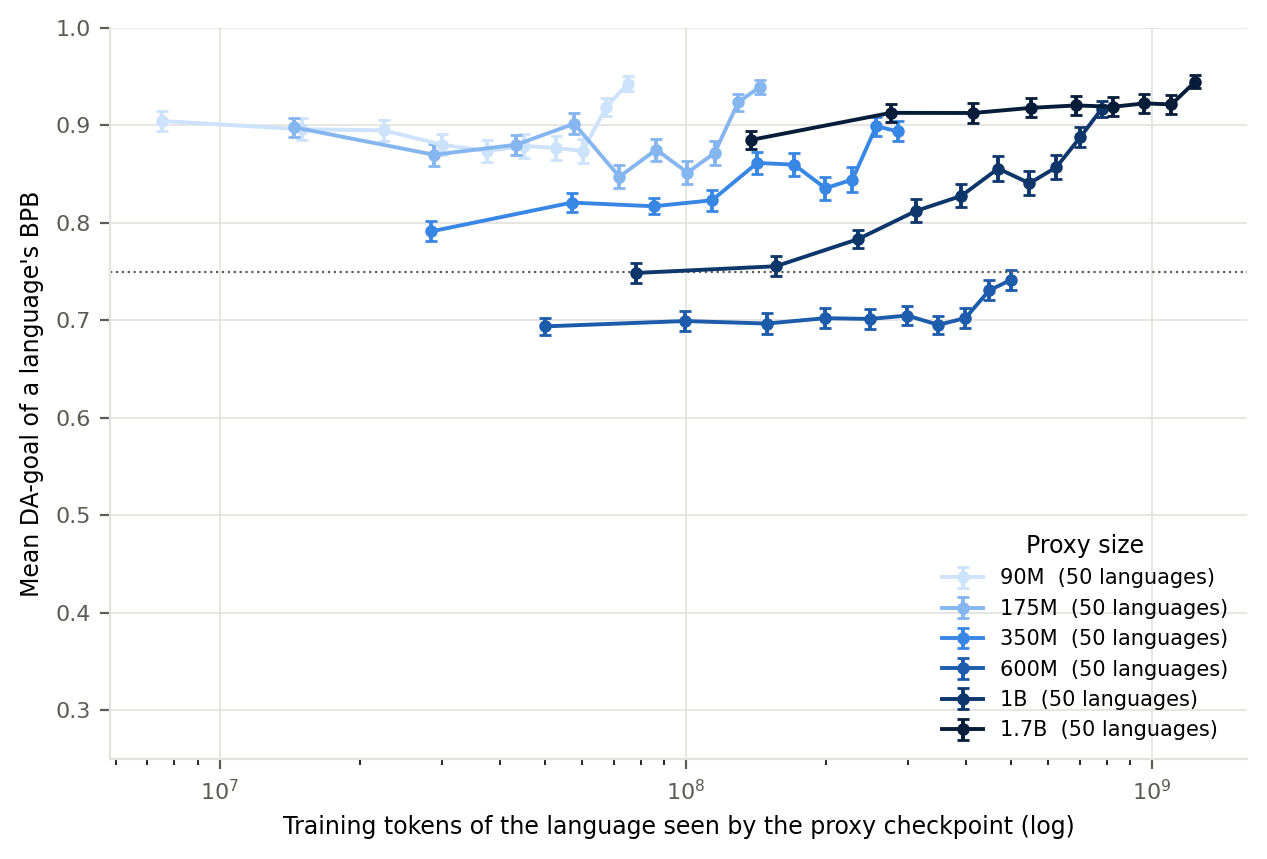
\includegraphics[width=\textwidth,height=0.36\textheight,keepaspectratio]{figures/app_rq02_da_goal_multi_axes_bpb.png}
% source: src/signal-and-noise/analysis/rq02_da_vs_train_tokens/pretraining/predictivity_seeds/da_goal_multi_axes_across_langs_bpb_paper.png
\captionof{figure}{\textbf{The 600M rung is the outlier, not the smallest proxy.} Mean DA-goal over the bits per byte of the 50 trained languages against the training tokens of the language that the checkpoint had seen (log scale). There is one line per proxy size, a darker blue for a larger size, and one point per evaluated tenth of the run. The x position is the geometric mean over languages, the bars give the standard error over languages and the dotted line marks 0.75.}
\label{fig:app_rq02_da_vs_train_tokens}
\end{minipage}
}]
